% -*- coding=utf-8 -*-
% !TEX TS-program = xelatex
% !TEX encoding = UTF-8 Unicode
% ============================================================================
% 文件名称：boyogala-main.tex
% 文件用途：江苏科技大学本科毕业设计（论文）LaTeX 模板主控文件
% 编译引擎：XeLaTeX + Biber + XeLaTeX + XeLaTeX（推荐使用 latexmk -xelatex）
% 规范依据：《江苏科技大学本科学位论文撰写要求及格式规范》（2021.12）及 justbks.md
% 设计目标：以精简无冗余的代码结构，实现完全符合学校规范、跨平台兼容且快速编译的排版
% ============================================================================

% ----------------------------------------------------------------------------
% 1. 文档类声明
% ----------------------------------------------------------------------------
% ctexbook     : CTeX 提供的中文书籍文档类，原生支持“章(chapter)-节(section)-条(subsection)”结构
% twoside      : 启用双面打印模式，奇偶页自动交换内外侧页边距（奇数页左28mm/右25mm，偶数页左25mm/右28mm）
% 12pt         : 设置基础正文字号为 12pt（对应中文“小四号”字，规范 4.2 节硬性要求）
% openright    : 双面排版下新章默认从右侧奇数页起始（前置摘要等部分通过局部重定义取消空白页）
% AutoFakeBold : 开启全局伪粗体支持，使无独立粗体字库的楷体、仿宋支持 \bfseries 加粗
% fontset=none : 禁用 ctexbook 默认操作系统/宏包字库探测，所有字体统一由 boyogala-setting.tex 从本地 font/ 目录加载
\documentclass[twoside,12pt,openright,AutoFakeBold,fontset=none]{ctexbook}

% ----------------------------------------------------------------------------
% 2. 载入全局导言区配置文件
% ----------------------------------------------------------------------------
% 集中管理宏包加载、页面几何、字体回退、页眉页脚、标题目录样式、参考文献、图表算法及数学环境
% 注：不再加载 zhlineskip 宏包，避免其覆盖规范要求的“固定值 20 磅”行距并减少每段钩子的编译开销
% -*- coding=utf-8 -*-
% ============================================================================
% 文件名称：boyogala-setting.tex
% ============================================================================
% ============================================================================
% 1. 核心宏包按需加载（已去除与 ctexbook / unicode-math 冲突或冗余的旧式 Type1 字体包）
% ============================================================================
\usepackage{wallpaper}                          % 封面及内封整页 PDF 底图铺设支持（提供 \ThisTileWallPaper）
\usepackage{amsmath,mathtools,amsthm}           % 数学公式增强与定理环境核心支持（在 unicode-math 之前加载）
\usepackage{etoolbox}                           % 编译期钩子工具（提供 \apptocmd、\AtBeginEnvironment 等补丁命令）
\usepackage{xcolor}                             % 增强型颜色支持（支持 listings 代码框中 gray!30、green!70!black 等混色语法）
\usepackage{fancyhdr}                           % 自定义页眉与页脚样式（实现奇偶页页眉文字、装饰线与居中页码）
\usepackage{geometry}                           % 页面版心尺寸、四周边距、装订线与页眉页脚空间精确控制
\usepackage{fontspec}                           % XeLaTeX OpenType/TrueType 本地字体路径与字重精确绑定支持
\usepackage{unicode-math}                       % 现代 OpenType 数学排版引擎（完全替代旧式 8-bit amsfonts/amssymb/bm/wasysym）
\usepackage{setspace}                           % 局部行距调节支持（提供声明页 \begin{spacing}{2.0} 与文献 \setstretch）
\usepackage{indentfirst}                        % 确保各章节标题后的第一段默认首行缩进
\usepackage{titletoc}                           % 目录条目格式定制（提供 \titlecontents 控制缩进、字体与引导点线）
\usepackage[inline]{enumitem}                   % 列表环境间距与行内列表定制（提供 \setlist 全局压缩列表空白）
\usepackage{graphicx,ragged2e}                  % 插图加载（\includegraphics、\graphicspath）与对齐辅助支持
\usepackage{subcaption}                         % 分图（subfigure / \subcaptionbox）排版与独立分图题注支持
\usepackage{bicaption}                          % 图表双语题注支持（提供 \bicaption 同时输出中英文双行图题/表题）
\usepackage{longtable,booktabs}                 % 跨页长表格（longtable）与标准三线表（\toprule/\midrule/\bottomrule）支持
\usepackage{listings}                           % 源代码清单排版、语法高亮、自动换行与阴影外框支持
\usepackage[plainruled,linesnumbered,algochapter]{algorithm2e} % 算法伪代码排版：三线风格、显示行号、按章编号
\usepackage{hyperref}                           % 交叉引用超链接与 PDF 书签大纲自动生成

% ============================================================================
% 2. 行间数学公式上下间距精调
% ============================================================================
% 定义紧凑的行间公式（display math）上下弹性间距，避免 20pt 正文行距下公式前后空白过大
\newcommand{\setmydisplayskip}{%
  \setlength{\abovedisplayskip}{3pt plus 1pt minus 1pt}%       % 长行间公式上方间距设为 3pt（可伸缩 ±1pt）
  \setlength{\belowdisplayskip}{3pt plus 1pt minus 1pt}%       % 长行间公式下方间距设为 3pt（可伸缩 ±1pt）
  \setlength{\abovedisplayshortskip}{3pt plus 1pt minus 1pt}%  % 前行文字较短时行间公式上方间距设为 3pt
  \setlength{\belowdisplayshortskip}{3pt plus 1pt minus 1pt}%  % 前行文字较短时行间公式下方间距设为 3pt
}
% 将公式间距设置挂载到 \normalsize 末尾，防止切换字号时被 LaTeX 重置为默认值
\apptocmd{\normalsize}{\setmydisplayskip}{}{}

% ============================================================================
% 3. 纸张尺寸、页边距、字体回退与页眉页脚样式（对应规范 3.2、4.1、4.2、4.4 节）
% ============================================================================
% 规范要求：A4 纸（210mm×297mm）双面打印；上 30mm、下 25mm、内侧（装订侧）28mm、外侧 25mm；
%           页眉距上缘约 20mm，页脚距下缘约 17.5mm
\geometry{%
  paperwidth  = 210mm,                          % 标准 A4 纸张宽度 210mm
  paperheight = 297mm,                          % 标准 A4 纸张高度 297mm
  twoside,                                      % 双面奇偶页对称交换内外边距（奇数页左28mm右25mm，偶数页左25mm右28mm）
  top         = 30mm,                           % 正文版心上边距 30mm
  bottom      = 25mm,                           % 正文版心下边距 25mm
  inner       = 28mm,                           % 装订侧（内侧）边距 28mm
  outer       = 25mm,                           % 切口侧（外侧）边距 25mm
  headheight  = 24pt,                           % 页眉盒子高度 24pt（约 8.4mm，消除 fancyhdr 高度不足警告）
  headsep     = 5.8mm,                          % 页眉基线至正文顶部间距 5.8mm（使页眉视觉位置距纸张上缘约 20mm）
  footskip    = 7.5mm                           % 正文底部至页脚基线间距 7.5mm（25mm - 7.5mm = 17.5mm，契合规范页脚位置）
}

% ----------------------------------------------------------------------------
% 3.1 本地字完备（Self-Contained）全套字体精确绑定（仅从 font/ 目录加载，零系统与第三方字库依赖）
% ----------------------------------------------------------------------------
% [1] 西文衬线主字体（\rmfamily）：采用 STI Pub 学术出版联盟最新研发的 STIX Two Text (v2.13)
%     兼具经典 Times 衬线风格与更高的 x-height 阅读舒适度，与下方 STIX Two Math 数学字体同源无缝衔接
\setmainfont{STIXTwoText-Regular.ttf}[          % 直接指定本地文件名，防止 fontspec 检索系统或 TeX Live 外部配置
  Path           = font/,                       % 强制仅从项目本地 font/ 目录检索字体文件，绝不调用操作系统字库
  BoldFont       = STIXTwoText-Bold.ttf,        % 粗体绑定 font/STIXTwoText-Bold.ttf
  ItalicFont     = STIXTwoText-Italic.ttf,      % 斜体绑定 font/STIXTwoText-Italic.ttf
  BoldItalicFont = STIXTwoText-BoldItalic.ttf   % 粗斜体绑定 font/STIXTwoText-BoldItalic.ttf
]

% [2] 西文无衬线字体（\sffamily）：采用 Adobe 最新第 3 代开源无衬线字体 Source Sans 3 (v3.052)
%     与中文思源黑体（Source Han Sans CN）为官方同源西文搭档，笔画黑度与字面率高度一致
\setsansfont{SourceSans3-Regular.otf}[          % 直接指定本地常规正体文件名 font/SourceSans3-Regular.otf
  Path           = font/,                       % 强制仅从项目本地 font/ 目录检索字体文件
  BoldFont       = SourceSans3-Bold.otf,        % 粗体绑定 font/SourceSans3-Bold.otf
  ItalicFont     = SourceSans3-It.otf,          % 斜体绑定 font/SourceSans3-It.otf
  BoldItalicFont = SourceSans3-BoldIt.otf       % 粗斜体绑定 font/SourceSans3-BoldIt.otf
]

% [3] 代码与西文等宽字体（\ttfamily）：采用 JetBrains 专为开发者设计的 JetBrains Mono (v2.304)
%     四字重齐全，原生内置完整希腊字母（如 Julia/Python 代码中的 \lambda），彻底避免回退系统或第三方包字体
\setmonofont{JetBrainsMono-Regular.ttf}[        % 直接指定本地文件名，杜绝触发 TeX Live 中 jetbrainsmono.fontspec
  Path           = font/,                       % 强制仅从项目本地 font/ 目录检索字体文件
  BoldFont       = JetBrainsMono-Bold.ttf,      % 粗体绑定 font/JetBrainsMono-Bold.ttf
  ItalicFont     = JetBrainsMono-Italic.ttf,    % 斜体绑定 font/JetBrainsMono-Italic.ttf
  BoldItalicFont = JetBrainsMono-BoldItalic.ttf,% 粗斜体绑定 font/JetBrainsMono-BoldItalic.ttf
  Scale          = MatchLowercase,              % 自动匹配正文小写字母高度，使行内代码与代码清单视觉比例协调
  Ligatures      = TeXOff                       % 关闭 TeX 传统连字（防止代码中 -- 或 '' 被合并为破折号或引号）
]

% [4] 数学公式字体（unicode-math）：采用顶级学术数学字体 STIX Two Math (v2.13, 6760 字形)
%     完整涵盖拉丁/希腊正斜体、粗体向量(\mathbf/\symbf)、空心黑板粗体(\mathbb)、花体(\mathcal)、
%     多级定界符及复选框符号，彻底摆脱 TeX 传统 Type1 (CMMI/CMSY/MSAM/MSBM/wasy) 第三方宏包字体
\setmathfont{STIXTwoMath-Regular.ttf}[          % 设置全局主数学字体为本地 STIXTwoMath-Regular.ttf
  Path           = font/                        % 强制仅从项目本地 font/ 目录加载
]
\setmathfont{STIXTwoMath-Regular.ttf}[          % 针对花体 \mathcal 与粗花体 \mathbfcal 单独启用 ss01 样式集
  Path           = font/,                       % 强制仅从项目本地 font/ 目录加载
  range          = {\mathcal,\mathbfcal},       % 作用范围限定为 \mathcal 与 \mathbfcal（保留 \mathscr 为手写花体）
  StylisticSet   = 1                            % 启用更符合国内数学教材习惯的经典正统花体字形
]
\setmathfont{XITSMath-Bold.otf}[                % 设置粗体数学版本（\boldmath）专用字体
  Path           = font/,                       % 强制仅从项目本地 font/ 目录加载
  version        = bold                         % 绑定至 bold 数学字重版本，杜绝伪粗体数学公式告警
]
\providecommand{\bm}[1]{\symbf{#1}}             % 兼容传统 \bm 粗体向量写法，直接映射为 OpenType 原生数学粗体符号

% [5] 中文主字体与四大家族字体（宋体、黑体、楷体、仿宋）：全部限定从本地 font/ 目录加载最新开源精品字库
%     - 宋体：Noto Serif CJK SC（思源宋体 v2.003，满配 65,535 字形，含 Regular 与原生 Bold 双字重，生僻字全覆盖）
%     - 黑体：Source Han Sans CN（思源黑体 v2.004，31,036 字形，含 Regular 与原生 Bold 双字重，标题庄重清晰）
%     - 楷体：LXGW WenKai（霞鹜文楷 2026 最新 v1.530，47,336 字形，含扩展 A 区汉字，兼具传统笔意与现代阅读舒适度）
%     - 仿宋：Zhuque Fangsong（朱雀仿宋 v0.212，13,805 字形，基于民国经典铅印仿宋重绘，字形秀丽稳健）
\setCJKmainfont{NotoSerifCJKsc-Regular.otf}[    % 设置中文默认主衬线字体为思源宋体 Regular
  Path           = font/,                       % 强制仅从项目本地 font/ 目录加载
  BoldFont       = NotoSerifCJKsc-Bold.otf,     % 中文 \bfseries 加粗直接调用原生思源宋体 Bold（非描边伪粗体）
  ItalicFont     = LXGWWenKai-Regular.ttf,      % 中文 \itshape 斜体自动映射为霞鹜文楷
  BoldItalicFont = NotoSerifCJKsc-Bold.otf      % 中文粗斜体映射为思源宋体 Bold
]
\setCJKsansfont{SourceHanSansCN-Regular.otf}[   % 设置中文默认无衬线字体为思源黑体 Regular
  Path           = font/,                       % 强制仅从项目本地 font/ 目录加载
  BoldFont       = SourceHanSansCN-Bold.otf,    % 无衬线加粗直接调用原生思源黑体 Bold
  ItalicFont     = LXGWWenKai-Regular.ttf       % 无衬线斜体映射为霞鹜文楷
]
\setCJKmonofont{ZhuqueFangsong-Regular.ttf}[    % 设置中文默认等宽字体为朱雀仿宋（用于代码注释等宽环境）
  Path           = font/,                       % 强制仅从项目本地 font/ 目录加载
  AutoFakeBold   = 2.0,                         % 为单字重仿宋启用适度伪粗体支持
  ItalicFont     = LXGWWenKai-Regular.ttf       % 等宽斜体映射为霞鹜文楷
]

% 显式声明 zhsong / zhhei / zhkai / zhfs 四大中文字族及对应切换命令（配合文档类 fontset=none 实现 100% 本地化）
\setCJKfamilyfont{zhsong}{NotoSerifCJKsc-Regular.otf}[  % 注册“宋体”字族 zhsong
  Path           = font/,                       % 强制仅从本地 font/ 目录加载
  BoldFont       = NotoSerifCJKsc-Bold.otf,     % 宋体加粗调用原生思源宋体 Bold（如声明页小二宋体加粗标题）
  ItalicFont     = LXGWWenKai-Regular.ttf       % 宋体斜体调用霞鹜文楷
]
\setCJKfamilyfont{zhhei}{SourceHanSansCN-Regular.otf}[  % 注册“黑体”字族 zhhei
  Path           = font/,                       % 强制仅从本地 font/ 目录加载
  BoldFont       = SourceHanSansCN-Bold.otf     % 黑体加粗调用原生思源黑体 Bold
]
\setCJKfamilyfont{zhkai}{LXGWWenKai-Regular.ttf}[       % 注册“楷体”字族 zhkai
  Path           = font/,                       % 强制仅从本地 font/ 目录加载
  AutoFakeBold   = 2.0                          % 楷体加粗启用伪粗体支持
]
\setCJKfamilyfont{zhfs}{ZhuqueFangsong-Regular.ttf}[    % 注册“仿宋”字族 zhfs
  Path           = font/,                       % 强制仅从本地 font/ 目录加载
  AutoFakeBold   = 2.0                          % 仿宋加粗启用伪粗体支持
]
\DeclareDocumentCommand{\songti}{}{\CJKfamily{zhsong}}  % 定义 \songti 切换至本地思源宋体
\DeclareDocumentCommand{\heiti}{}{\CJKfamily{zhhei}}    % 定义 \heiti 切换至本地思源黑体
\DeclareDocumentCommand{\kaishu}{}{\CJKfamily{zhkai}}   % 定义 \kaishu 切换至本地霞鹜文楷
\DeclareDocumentCommand{\fangsong}{}{\CJKfamily{zhfs}}  % 定义 \fangsong 切换至本地朱雀仿宋

% 正文全局默认排版参数（规范 4.2 节硬性要求：小四号宋体，行间距固定值 20 磅，标准字距）
\AtBeginDocument{%
  \linespread{1}\songti\fontsize{12pt}{20pt}\selectfont % 文档开始时锁定倍率为1、宋体、字号12pt（小四）、基线行距固定20pt
  \DeclareDocumentCommand{\square}{}{\ensuremath{\char"2610}}%     % 将 \square 绑定为 STIXTwoMath 内置空心复选框 ☐ (U+2610)
  \DeclareDocumentCommand{\CheckedBox}{}{\ensuremath{\char"2611}}% % 将 \CheckedBox 绑定为 STIXTwoMath 内置打钩复选框 ☑ (U+2611)
}
\raggedbottom                                   % 关闭页面垂直方向强制拉伸对齐，防止段落或标题间被拉出异常空白
\setlength{\parindent}{2em}                     % 正文段落首行缩进固定为 2 个汉字宽度（2em）
\setlength{\emergencystretch}{3em}              % 允许行内额外紧急伸展 3em，消除中英文与行内公式混排时的右侧溢出（Overfull \hbox）

% 前置部分（摘要、目录页）使用的 plain 页面样式：无页眉、无装饰线，仅页脚居中显示五号页码
\fancypagestyle{plain}{%
  \fancyhf{}%                                   % 清空默认页眉与页脚内容
  \fancyfoot[C]{\zihao{5}\thepage}%             % 页脚居中打印五号（10.5pt）页码
  \renewcommand{\headrulewidth}{0pt}%           % 将页眉默认横线宽度设为 0pt
  \renewcommand{\headrule}{}%                   % 清空页眉装饰线绘制命令，确保摘要和目录页顶部无横线
}

% 正文及后置部分（章节、结论、参考文献、致谢、附录）通用的页眉页脚宏定义（规范 4.4 节）
\newcommand{\justheaderfooter}{%
  \fancyhf{}%                                   % 清空所有页眉与页脚区域
  \fancyfoot[C]{\zihao{5}\thepage}%             % 奇偶页页脚均居中显示五号（10.5pt）Times New Roman 页码
  \fancyhead[CE,CO]{\zihao{5}\songti 江苏科技大学本科毕业设计（论文）}% % 偶数页(CE)与奇数页(CO)页眉均居中显示五号宋体规定字样
  \renewcommand{\headrulewidth}{0pt}%           % 关闭 fancyhdr 默认贴底横线，改用下方自定义位置横线
  \renewcommand{\headrule}{%                    % 自定义页眉下方实线：线宽等于版心宽度 \headwidth，粗细为 0.8pt
    \makebox[0pt][l]{\rule[.7\baselineskip]{\headwidth}{0.8pt}}%
  }%
}
% 定义名为 myfancy 的正文页面样式，直接调用 \justheaderfooter
\fancypagestyle{myfancy}{\justheaderfooter}

% ============================================================================
% 4. 正文四级标题层级格式与间距设置（对应规范 3.5、4.2、4.7 节）
% ============================================================================
% 规范要求：以正文 20pt 行距为基准，章段前/段后 1.5 行(30pt)，节 1.0 行(20pt)，条/款 0.5 行(10pt)
\ctexset{
  chapter = {                                   % 一级标题（章）：如“第 1 章 绪论”
    name       = {第,章},                       % 章号前后缀设为“第 X 章”
    number     = \arabic{chapter},              % 章序采用阿拉伯数字（1, 2, 3...）
    format     = \heiti\zihao{-3}\centering,    % 字体字号：小三号（15pt）黑体，居中排写
    beforeskip = 30pt,                          % 段前间距 1.5 行（1.5 × 20pt = 30pt）
    afterskip  = 30pt,                          % 段后间距 1.5 行（1.5 × 20pt = 30pt）
    fixskip    = true                           % 抑制 ctex 默认额外顶部空白，使段前段后间距精确生效
  },
  section = {                                   % 二级标题（节）：如“1.1 研究背景”
    format     = \heiti\zihao{4}\raggedright,   % 字体字号：四号（14pt）黑体，左对齐顶格书写
    beforeskip = 20pt,                          % 段前间距 1.0 行（1.0 × 20pt = 20pt）
    afterskip  = 20pt,                          % 段后间距 1.0 行（1.0 × 20pt = 20pt）
    fixskip    = true                           % 精确控制节标题上下间距
  },
  subsection = {                                % 三级标题（条）：如“1.1.1 国内外现状”
    format     = \heiti\zihao{-4}\raggedright,  % 字体字号：小四号（12pt）黑体，左对齐顶格书写
    beforeskip = 10pt,                          % 段前间距 0.5 行（0.5 × 20pt = 10pt）
    afterskip  = 10pt,                          % 段后间距 0.5 行（0.5 × 20pt = 10pt）
    fixskip    = true                           % 精确控制条标题上下间距
  },
  subsubsection = {                             % 四级标题（款）：如“1.1.1.1 具体方法”
    format     = \heiti\zihao{-4}\raggedright,  % 字体字号：小四号（12pt）黑体，左对齐顶格书写
    beforeskip = 10pt,                          % 段前间距 0.5 行（10pt）
    afterskip  = 10pt,                          % 段后间距 0.5 行（10pt）
    fixskip    = true                           % 精确控制款标题上下间距
  }
}
% 设置章节自动编号深度为 3（即编号至四级标题 subsubsection：1.1.1.1）
\setcounter{secnumdepth}{3}

% ============================================================================
% 5. 目录格式定制（对应规范 2.1.4、3.4、4.6 节及附录 9）
% ============================================================================
% 规范要求：目录题头居中；仅列至三级标题（章、节、条）；章条目用小四号黑体顶格，
%           节、条用小四号宋体分别缩进 1 格、2 格；右侧点线引导并右对齐页码
\renewcommand{\contentsname}{目\hspace{2em}录}  % 目录标题设为“目　录”，中间空两格
\setcounter{tocdepth}{2}                        % 目录收录深度设为 2（仅显示 chapter、section、subsection 三级）

% 一级目录条目（chapter 章）：顶格排写，小四号（12pt）黑体，行距 16.5pt
\titlecontents{chapter}[4em]                    % 标题文本左端距版心左缘 4em（预留给“第X章”编号盒）
  {\heiti\fontsize{12pt}{16.5pt}\selectfont}    % 章目录字体：小四号（12pt）黑体，固定行高 16.5pt
  {\contentslabel{4em}}                         % 有编号章：在 4em 宽盒子内左对齐输出“第X章”使其顶格
  {\hspace*{-4em}}                              % 无编号章（摘要、结论、参考文献、致谢、附录）：回退 4em 使其顶格
  {~\titlerule*[0.6pc]{$.$}~\contentspage}      % 标题与页码之间填充间距为 0.6pc 的圆点引导线，页码居右对齐

% 二级目录条目（section 节）：相对一级标题缩进 1 个汉字，小四号（12pt）宋体
\titlecontents{section}[3em]                    % 标题文本左端距版心左缘 3em（1em 缩进 + 2em 节号盒）
  {\songti\fontsize{12pt}{16.5pt}\selectfont}   % 节目录字体：小四号（12pt）宋体，行高 16.5pt
  {\contentslabel{2em}}                         % 节编号（如 1.1）占宽 2em，左起位置距左缘 3em - 2em = 1em（缩进一格）
  {\hspace*{-2em}}                              % 无编号节回退 2em
  {~\titlerule*[0.6pc]{$.$}~\contentspage}      % 圆点引导线及右对齐页码

% 三级目录条目（subsection 条）：相对一级标题缩进 2 个汉字，小四号（12pt）宋体
\titlecontents{subsection}[6em]                 % 标题文本左端距版心左缘 6em
  {\songti\fontsize{12pt}{16.5pt}\selectfont}   % 条目录字体：小四号（12pt）宋体，行高 16.5pt
  {\contentslabel{3em}}                         % 条编号（如 1.1.1）占宽 3em，缩进展示清晰层次
  {\hspace*{-2em}}                              % 无编号条回退 2em
  {~\titlerule*[0.6pc]{$.$}~\contentspage}      % 圆点引导线及右对齐页码

% ============================================================================
% 6. 参考文献设置（对应规范 2.2.4、3.6、3.13、4.2 节及附录 6）
% ============================================================================
% 规范要求：按正文首次引用顺序编码；正文中右上角方括号上标引用（\upcite）；文献列表采用五号宋体
\usepackage[
  backend=biber,                                % 指定使用 Biber 后端处理 UTF-8 中英文混合文献数据
  style=gb7714-2025,                            % 加载项目根目录附带的国标 GB/T 7714-2025 著录与引用样式
  sorting=none,                                 % 严格按照文献在正文中首次被引用的先后顺序编号排列
  gbnamefmt=lowercase,                          % 西文作者姓名采用首字母大写、其余小写的常规大小写格式
  gbalign=gb7714-2025                           % 序号顶格对齐，换行后与作者名首字对齐（符合规范附录 6 第 7 条）
]{biblatex}
\addbibresource{ref.bib}                        % 挂载根目录下的 ref.bib 参考文献数据库文件
\AtBeginBibliography{\songti\zihao{5}\setstretch{1.0}} % 将参考文献列表区域字体统一设为五号（10.5pt）宋体、单倍紧凑行距

% ============================================================================
% 7. 数学定理、引理、推论、定义、例、注与证明环境
% ============================================================================
% 定理、定义、引理、推论共享按章编号计数器（如“定理 2.1”后紧接“引理 2.2”），标题首行缩进 2em
\theoremstyle{definition}                       % 切换为正体定理样式：使定理正文保持小四宋体正体，消除中文斜体加粗缺失警告
\newtheorem{theorem}{\hskip 2em 定理}[chapter]       % 定义按章编号的“定理”环境
\newtheorem{definition}[theorem]{\hskip 2em 定义}    % 定义与 theorem 共享编号的“定义”环境
\newtheorem{lemma}[theorem]{\hskip 2em 引理}         % 定义与 theorem 共享编号的“引理”环境
\newtheorem{corollary}[theorem]{\hskip 2em 推论}     % 定义与 theorem 共享编号的“推论”环境
\newtheorem{example}{\hskip 2em 例}[chapter]         % 定义按章独立编号的“例”环境
\newtheorem{remark}{\hskip 2em 注}[chapter]          % 定义按章独立编号的“注”环境
\renewcommand{\proofname}{\hskip 2em \bfseries 证明}  % 将 amsthm 默认证明环境题头改为首行缩进 2em 的加粗“证明”

% ============================================================================
% 8. 数学公式按章编号（对应规范 3.10、4.8 节）
% ============================================================================
% 规范要求：公式序号按章编排，如第 1 章第一个公式为 (1.1)，居于右侧靠近版心右边线
\numberwithin{equation}{chapter}

% ============================================================================
% 9. 插图、插表双语题注、表格字体与列表样式（对应规范 3.11、3.12、4.2 节）
% ============================================================================
% 规范要求：图题置于图下、表题置于表上，居中排写；图题、表题、表头及表内文字均采用五号宋体；
%           图序/表序与图名/表名之间空一格
\DeclareCaptionFont{captionsong}{\songti\zihao{5}}   % 声明中文题注专用字体：五号（10.5pt）宋体
\DeclareCaptionFont{captiontimes}{\rmfamily\zihao{5}}% 声明英文题注专用字体：五号（10.5pt）Times New Roman
\captionsetup{
  labelsep=quad,                                % 图表序号（如“图 1.1”）与标题文字之间空一格（1em）
  justification=centering,                      % 题注整体居中排写
  singlelinecheck=true,                         % 单行题注自动居中
  skip=6pt                                      % 题注与图表主体之间的垂直间距设为 6pt
}
\captionsetup[bi-first]{font=captionsong,labelfont=captionsong}     % 双语题注第一行（中文）应用五号宋体
\captionsetup[bi-second]{font=captiontimes,labelfont=captiontimes}  % 双语题注第二行（英文）应用五号新罗马体
\AtBeginEnvironment{figure}{\captionsetup[bi-second]{name=Fig.}}    % 插图英文题注前缀设为“Fig.”（匹配规范附录 5）
\AtBeginEnvironment{table}{\captionsetup[bi-second]{name=Table}}    % 插表英文题注前缀设为“Table”（匹配规范附录 4）

% 全局列表环境（itemize / enumerate / description）紧凑间距配置
\setlist{
  topsep=0.3em,                                 % 列表环境顶部及底部与上下文段落的垂直间距
  partopsep=0pt,                                % 列表前有空行时不额外增加顶部垂直空白
  itemsep=0ex plus 0.1ex,                       % 相邻列表项之间的垂直间距
  parsep=0pt,                                   % 同一列表项内部段落之间的垂直间距
  leftmargin=1.5em,                             % 列表左边界缩进量
  rightmargin=0em,                              % 列表右边界缩进量
  labelsep=0.5em,                               % 列表序号标签与文字之间的水平间距
  labelwidth=2em                                % 列表序号标签盒宽度
}

\graphicspath{{figure/}{./}}                    % 设置默认图片搜索路径：优先检索 figure/ 子目录及项目根目录
\AtBeginEnvironment{table}{\songti\zihao{5}}    % 进入普通浮动表格环境时自动切换为规范要求的五号宋体
\AtBeginEnvironment{longtable}{\songti\zihao{5}}% 进入跨页长表格环境时自动切换为规范要求的五号宋体

% ============================================================================
% 10. 源代码清单排版配置（listings 宏包，适用于正文或附录程序代码）
% ============================================================================
\renewcommand{\lstlistingname}{代码}            % 将代码清单题注前缀设为中文“代码”（如“代码 1.1”）
\lstset{
  language=python,                              % 默认语法高亮语言设为 Python（可在具体环境中通过 language= 覆盖）
  frame=shadowbox,                              % 绘制带右下角立体阴影的矩形外框
  rulesepcolor=\color{gray!30},                 % 阴影边框填充为 30% 浅灰色
  framesep=4pt,                                 % 代码框线与内部文字的基础内边距
  xleftmargin=1.8em,                            % 代码框整体左缩进 1.8em，为左侧行号预留充足空间
  framexleftmargin=0pt,                         % 左边框与代码对齐，使行号清晰排布于左框线外侧而不压线
  framexrightmargin=4pt,                        % 边框向右侧扩展 4pt
  framextopmargin=4pt,                          % 边框向上方扩展 4pt
  framexbottommargin=4pt,                       % 边框向下方扩展 4pt
  keywordstyle=\color{blue},                    % 语言关键字高亮为蓝色
  commentstyle=\color{green!70!black},          % 代码注释高亮为深绿色
  stringstyle=\color{magenta},                  % 字符串字面量高亮为洋红色
  basicstyle=\ttfamily\small,                   % 代码主体采用小号（\small）JetBrains Mono 等宽字体
  breaklines=true,                              % 超长代码行自动折行，防止溢出右边距
  showstringspaces=false,                       % 不将字符串中的空格显示为特殊可见符号
  numbers=left,                                 % 在代码框左侧显示行号
  numberstyle=\tiny\color{gray},                % 行号采用微小字号（\tiny）灰色字体
  tabsize=4,                                    % 制表符 Tab 等效缩进为 4 个空格
  numbersep=8pt                                 % 行号与代码左框线之间的间距设为 8pt，杜绝与左框线重叠
}

% ============================================================================
% 11. 交叉引用与超链接属性设置（打印版友好配置）
% ============================================================================
\hypersetup{
  colorlinks=true,                              % 启用文字颜色链接模式，去除链接周围难看的彩色方框
  urlcolor=black,                               % 外部网页链接设为纯黑色，保证双面打印清晰统一
  linkcolor=black,                              % 目录、公式、图表等内部交叉引用链接设为纯黑色
  anchorcolor=black,                            % 锚点文本颜色设为纯黑色
  citecolor=black                               % 参考文献引用标注链接设为纯黑色
}

% ============================================================================
% 12. 算法伪代码环境（algorithm2e）双语题注与三线表风格定制
% ============================================================================
\makeatletter                                   % 开启 @ 字符作为内部宏名字符权限
\newcommand{\algoenname}{\textbf{Algo.}}        % 定义算法英文题注前缀为加粗的“Algo.”
\renewcommand{\algorithmcfname}{算法}           % 将算法中文题注前缀重定义为“算法”
\setlength\AlCapSkip{1.2ex}                     % 设置算法题注与顶部横线之间的间距为 1.2ex
\SetAlgoSkip{1pt}                               % 设置算法浮动体与上下文正文之间的额外间距
\setlength{\algoheightruledefault}{1.5pt}       % 设置算法顶部与标题下方横线的默认线宽为 1.5pt

% 设置算法编号格式为“章号-序号”（例如第 4 章第 1 个算法显示为“4-1”）
\expandafter\ifx\csname algocf@within\endcsname\relax
  \renewcommand\thealgocf{\@arabic\c@algocf}    % 若未启用按章编号，则直接输出阿拉伯数字序号
\else
  \renewcommand\thealgocf{\csname the\algocf@within\endcsname-\@arabic\c@algocf} % 启用按章编号时输出“章-序号”
\fi

% 重定义 algorithm2e 内部题注生成宏，使中英文双语算法标题整体居中、行距 1.5em 且不超出算法框宽度
\renewcommand{\algocf@makecaption}[2]{%
  \noindent\parbox[t]{\hsize}{%                 % 顶格创建与算法框等宽的段落盒，消除首行缩进与边距叠加导致的 42.4pt 溢出
    \centering                                  % 盒内题注文字居中对齐
    \setlength{\baselineskip}{1.5em}%           % 中英文两行标题之间的基线间距设为 1.5em
    \AlCapFnt{}#1\algocf@typo~\AlCapFnt{}#2%    % 依次输出“算法 X-X”标签（#1）、空格与标题文本（#2）
  }%
}

% 定义算法双语题注命令 \AlgoBiCaption{中文算法名}{英文算法名}
\newcommand{\AlgoBiCaption}[2]{%
  \caption[#1]{#1\\ \algoenname\ \thealgocf~~#2}% % 第一行输出中文标题，换行后第二行输出“Algo. X-X  英文标题”
  \addcontentsline{aen}{algoen}{\protect\numberline{ }{#2}}% % 记录英文算法清单索引条目
}

% 重定义 plainruled 风格下算法底部的收尾横线粗细为 1.5pt，与顶部横线形成对称三线表风格
\def\@algocf@post@ruled{\kern\interspacealgoruled\hrule height1.5pt\relax}
% 同步 algorithm 内部 \linewidth 与 \hsize，消除算法内嵌套 itemize 列表时的 42.4pt 宽度溢出警告
\apptocmd{\@algocf@start}{\setlength{\linewidth}{\hsize}}{}{}
\makeatother                                    % 关闭 @ 字符权限

% 设置算法输入与输出关键字的中文显示名称
\SetKwInput{KwIn}{输入}                         % \KwIn{...} 显示为“输入：...”
\SetKwInput{KwOut}{输出}                        % \KwOut{...} 显示为“输出：...”

% ============================================================================
% 13. 常用数学算子与正体常数快捷命令（符合规范 3.8.3 节正斜体规定）
% ============================================================================
% 规范要求：函数名、微分算子 d、虚数单位 i、自然底数 e 等数学常量与算子一律采用正体
\renewcommand{\Re}{\operatorname{Re}}           % 复数实部算子 Re（正体）
\renewcommand{\Im}{\operatorname{Im}}           % 复数虚部算子 Im（正体）
\newcommand{\mi}{\mathrm{i}}                    % 正体虚数单位 i
\newcommand{\md}{\mathrm{d}}                    % 正体微分算子 d（如 \int f(x)\,\md x）
\newcommand{\me}{\mathrm{e}}                    % 正体自然对数底数 e（如 \me^{-x}）
\DeclareMathOperator{\argmin}{argmin}           % 极小值点算子 argmin（正体）
\DeclareMathOperator{\supp}{supp}               % 支集算子 supp（正体）
\DeclareMathOperator{\prox}{prox}               % 近端算子 prox（正体）
\DeclareMathOperator{\sign}{sign}               % 符号函数算子 sign（正体）


% ============================================================================
% 3. 论文文档主体开始
% ============================================================================
\begin{document}

  % --------------------------------------------------------------------------
  % 3.1 前置部分（一）：外封面、内封（扉页）、原创性声明与版权使用授权书
  % 规范要求：无页眉、无页脚页码，章节不编号
  % --------------------------------------------------------------------------
  \frontmatter                                  % 切换至前置部分模式：关闭章节自动编号（\chapter 不生成“第X章”）
  \pagestyle{empty}                             % 设置页面样式为空：隐去外封面、内封、声明及授权书的所有页眉与页码
  % -*- coding=utf-8 -*-
% ============================================================================
% 文件名称：chapter/boyogala1_cover.tex
% 文件用途：江苏科技大学本科毕业设计（论文）外封面与内封（扉页）
% 规范依据：《江苏科技大学本科学位论文撰写要求及格式规范》第 2.1.1、2.1.2、4.3 节及附录 7、8
% ============================================================================

% -------------------- 论文基本信息配置（请修改为个人信息） --------------------
\newcommand\studentId{你的学号}                                                 % 学生班级学号
\newcommand\thesisTitleCN{基于粒子群算法的第一和第二特征值及其单位特征向量的求解} % 中文论文题目（原则上不超过25字，不设副标题）
\newcommand\thesisTitleEN{Computation of the First and Second Eigenvalues and Their Corresponding Unit Eigenvectors Based on Particle Swarm Optimization} % 英文论文题目
\newcommand\thesisAuthor{你的名字}                                              % 学生姓名
\newcommand\supervisor{王俊}                                                    % 指导教师姓名
\newcommand\majorclass{信息与计算科学}                                          % 专业名称
\newcommand\institute{理学院}                                                   % 学院名称
\newcommand\thesisDateOne{2026 年 6 月}                                         % 外封面底部提交日期（阿拉伯数字年月）
\newcommand\thesisDateTwo{二零二六年六月}                                       % 内封底部提交日期（汉字数字年月）

% ============================================================================
% 第一页：外封面（规范附录 7：采用教务处统一封面底图 cover1.pdf，信息栏采用四号黑体）
% ============================================================================
{%
  \setlength{\parindent}{0pt}%                                                  % 取消封面段落首行缩进
  \ThisTileWallPaper{\paperwidth}{\paperheight}{figure/cover1.pdf}%             % 铺设学校统一外封面 PDF 底图
  \vspace*{13.5cm}%                                                             % 留出上方校徽与“本科毕业设计（论文）”大标题区域
  \begin{center}%
    \heiti\fontsize{14pt}{28pt}\selectfont                                      % 显式锁定四号黑体（14pt）与固定 28pt 行高，杜绝受外部行距影响
    \makebox[6em][r]{学\hspace{1.5em}院}\hspace{0.3em}%
    \underline{\makebox[15em][c]{\institute}}\par
    \makebox[6em][r]{专\hspace{1.5em}业}\hspace{0.3em}%
    \underline{\makebox[15em][c]{\majorclass}}\par
    \makebox[6em][r]{学生姓名}\hspace{0.3em}%
    \underline{\makebox[15em][c]{\thesisAuthor}}\par
    \makebox[6em][r]{班级学号}\hspace{0.3em}%
    \underline{\makebox[15em][c]{\studentId}}\par
    \makebox[6em][r]{指导教师}\hspace{0.3em}%
    \underline{\makebox[15em][c]{\supervisor}}\par
  \end{center}%
  \vfill                                                                        % 弹性填充垂直空白，将日期稳固锚定在封面第一页底部，绝不跨页
  \begin{center}%
    \heiti\fontsize{14pt}{20pt}\selectfont
    \makebox[5cm][c]{\thesisDateOne}\par                                        % 底部居中显示“2026 年 6 月”
  \end{center}%
  \vspace*{0.6cm}%                                                              % 底部留白缓冲
}

\newpage

% ============================================================================
% 第二页：内封 / 扉页（规范附录 8：中文题目二号黑体居中，英文题目 16pt 新罗马体居中，其余四号宋体居中）
% ============================================================================
{%
  \setlength{\parindent}{0pt}%                                                  % 取消内封段落首行缩进
  \ThisTileWallPaper{\paperwidth}{\paperheight}{figure/cover2.pdf}%             % 铺设内封 PDF 底图（含顶部四号宋体“江苏科技大学本科毕业论文”）
  \vspace*{2.5cm}%                                                              % 顶部标题与论文中文题目之间的间距
  \begin{center}%
    \makebox[15cm][c]{%
      \parbox{12.5cm}{%
        \centering\heiti\fontsize{22pt}{30pt}\selectfont                        % 中文题目：二号（22pt）黑体居中，行距 30pt
        \thesisTitleCN
      }%
    }\par
    \vspace{0.6cm}%                                                             % 中英文题目之间的垂直间距
    \makebox[15cm][c]{%
      \parbox{15cm}{%
        \centering\rmfamily\fontsize{16pt}{22pt}\selectfont                     % 英文题目：Times New Roman 16pt（三号）居中，行距 22pt
        \thesisTitleEN
      }%
    }\par
  \end{center}%

  \vspace*{3.6cm}%                                                              % 英文题目与署名区之间的垂直间距
  \begin{center}%
    \songti\fontsize{14pt}{24pt}\selectfont                                     % 署名区：四号（14pt）宋体居中，固定行距 24pt
    % 若所在学院要求内封同时打印学号，取消下一行注释即可：
    % 学生学号：\makebox[4.5em][l]{\studentId}\par
    学生姓名：\makebox[4.5em][l]{\thesisAuthor}\par
    指导教师：\makebox[4.5em][l]{\supervisor}\par
  \end{center}%

  \vfill                                                                        % 弹性填充垂直空白，将校名与日期稳固锚定在内封底部，绝不跨页
  \begin{center}%
    \songti\fontsize{14pt}{22pt}\selectfont                                     % 底部校名与日期：四号（14pt）宋体居中
    \makebox[5cm][c]{江苏科技大学}\par
    \vspace{0.35cm}%
    \makebox[5cm][c]{\thesisDateTwo}\par
  \end{center}%
  \vspace*{0.6cm}%                                                              % 底部留白缓冲
}
             % 载入外封面（figure/cover1.pdf 底图）与内封/扉页（figure/cover2.pdf 底图）
  % -*- coding=utf-8 -*-
% ============================================================================
% 文件名称：chapter/boyogala2_statement.tex
% 文件用途：江苏科技大学学位论文原创性声明与版权使用授权书
% 规范依据：《江苏科技大学本科学位论文撰写要求及格式规范》第 2.1 节及附录 8
% ============================================================================

% ============================================================================
% 第一页：学位论文原创性声明（小二宋体加粗居中标题，小四宋体 2.0 倍行距正文）
% ============================================================================
{%
  \setlength{\parindent}{2em}%
  \vspace*{2cm}%
  \begin{center}%
    {\songti\zihao{-2}\bfseries 江苏科技大学学位论文原创性声明\par}%
  \end{center}%
  \vspace{21pt}%

  \begin{spacing}{2.0}%
  {\songti\zihao{-4}%
  本人郑重声明：所呈交的学位论文，是本人在导师的指导下，独立进行研究工作所取得的成果。除文中已经注明引用的内容外，本论文不包含任何其他个人或集体已经发表或撰写过的作品成果。对本文的研究做出重要贡献的个人和集体，均已在文中以明确方式标明。

  本人完全意识到本声明的法律结果由本人承担。}
  \end{spacing}%

  \vspace{9em}%
  \begin{center}%
    {\songti\zihao{-4}%
    学位论文作者签名（手签）：\makebox[5em][c]{}\quad
    日期：\makebox[3em][c]{} 年 \makebox[1.5em][c]{} 月 \makebox[1.5em][c]{} 日}
  \end{center}%
}

\newpage

% ============================================================================
% 第二页：学位论文版权使用授权书（小二宋体加粗居中标题，小四宋体 2.0 倍行距正文）
% ============================================================================
{%
  \setlength{\parindent}{2em}%
  \vspace*{2cm}%
  \begin{center}%
    {\songti\zihao{-2}\bfseries 江苏科技大学学位论文版权使用授权书\par}%
  \end{center}%
  \vspace{21pt}%

  \begin{spacing}{2.0}%
  {\songti\zihao{-4}%
  本学位论文作者完全了解学校有关保留、使用学位论文的规定，同意学校保留并向国家有关部门或机构送交论文的复印件和电子版，允许论文被查阅和借阅。本人授权江苏科技大学可以将本学位论文的全部或部分内容编入有关数据库进行检索，可以采用影印、缩印或扫描等复制手段保存和汇编本学位论文。

  本学位论文属于：

  (1) 保密$\square$，在\hspace{3em}年解密后适用本授权书。

  (2) 不保密$\CheckedBox$。}
  \end{spacing}%

  \vspace{9em}%
  \begin{center}%
    \begin{tabular}{@{}p{0.48\textwidth}@{}p{0.48\textwidth}@{}}
      {\songti\zihao{-4}学位论文作者签名（手签）：\makebox[3em][c]{}} &
      {\songti\zihao{-4}指导教师签名（手签）：\makebox[3em][c]{}} \\[1.2em]
      {\songti\zihao{-4}日期：\makebox[2em][c]{} 年 \makebox[1.2em][c]{} 月 \makebox[1.2em][c]{} 日} &
      {\songti\zihao{-4}日期：\makebox[2em][c]{} 年 \makebox[1.2em][c]{} 月 \makebox[1.2em][c]{} 日}
    \end{tabular}%
  \end{center}%
}
         % 载入《学位论文原创性声明》与《学位论文版权使用授权书》

  % --------------------------------------------------------------------------
  % 3.2 前置部分（二）：中文摘要、英文摘要与目录
  % 规范要求：无正文页眉，页脚居中打印五号大写罗马数字页码（从 I 连续编号）
  % --------------------------------------------------------------------------
  \pagestyle{plain}                             % 启用前置部分 plain 样式：无页眉及装饰线，仅页脚居中显示五号页码
  \pagenumbering{Roman}                         % 将页码切换为大写罗马数字（I, II, III...），并将页码计数器重置为 1
  \let\cleardoublepage\clearpage                % 将双面强制奇数页换页改为普通换页，避免摘要、目录之间插入多余空白页
  % -*- coding=utf-8 -*-
% ============================================================================
% 文件名称：chapter/boyogala3_abstract_cn.tex
% 文件用途：中文摘要与关键词（规范 2.1.3、3.3、4.5 节：三号黑体题头，小四宋体固定 20pt 行距）
% ============================================================================
\chapter*{\texorpdfstring{\zihao{3}摘\quad 要}{摘要}}
\addcontentsline{toc}{chapter}{\texorpdfstring{摘\quad 要}{摘要}}

{\songti\fontsize{12pt}{20pt}\selectfont
主要工作是基于已有 Overleaf 模板，结合《江苏科技大学本科学位论文撰写要求及格式规范》，提供了一个结构精简、编译快速的江苏科技大学理工科本科生毕业设计（论文）\LaTeX 模板。为了让大家使用模板更加方便，本模板对于主文件与导言区配置文件的每一行代码都作了详细注释，并且优化了整体的宏包与排版结构，上手更加容易。
}

\par\vspace{\baselineskip}
\noindent
{\heiti\zihao{-4}关键词：}{\songti\zihao{-4}\LaTeX 模板；学位论文；江苏科技大学}

\clearpage
       % 载入中文摘要与关键词（起始页码为 I，自动写入目录）
  % -*- coding=utf-8 -*-
% ============================================================================
% 文件名称：chapter/boyogala4_abstract_en.tex
% 文件用途：英文摘要与关键词（规范 2.1.3、3.3、4.5 节：三号粗体 Abstract，小四新罗马体固定 20pt 行距）
% ============================================================================
\chapter*{\zihao{3}\bfseries Abstract}
\addcontentsline{toc}{chapter}{Abstract}

{\rmfamily\fontsize{12pt}{20pt}\selectfont
The main work of this article is based on the existing Overleaf template and the official formatting specification of Jiangsu University of Science and Technology (JUST), providing a concise and fast-compiling \LaTeX\ undergraduate thesis template. In order to make it more convenient for everyone to use the template, every line of code in the main and configuration files has been annotated in detail, and the overall structure has been optimized to make it easier to get started.
}

\par\vspace{\baselineskip}
\noindent
{\rmfamily\bfseries\zihao{-4}Key words: }{\rmfamily\zihao{-4}\LaTeX\ template; undergraduate thesis; JUST}

\clearpage
       % 载入英文摘要 Abstract 与 Key words（紧接中文摘要，例如页码为 II）

  \pagestyle{plain}                             % 确保目录页保持无页眉、仅页脚居中显示罗马数字页码的 plain 样式
  \tableofcontents                              % 自动生成目录（紧接英文摘要，例如页码为 III，仅收录至三级标题 subsection）
  \clearpage                                    % 结束目录最后1页并输出缓冲区内容
  \thispagestyle{plain}                         % 确保目录末尾页同样应用 plain 页码样式

  % --------------------------------------------------------------------------
  % 3.3 主体部分：绪论及各正文章节
  % 规范要求：页眉居中显示五号宋体“江苏科技大学本科毕业设计（论文）”及 0.8pt 下划线，
  %           页脚居中显示五号阿拉伯数字页码（从 1 重新开始连续编号）
  % --------------------------------------------------------------------------
  \mainmatter                                   % 切换至正文模式：开启章节阿拉伯数字编号，并将页码重置为阿拉伯数字 1
  \fancypagestyle{plain}{\justheaderfooter}     % 重定义章首页默认的 plain 样式为正文页眉页脚，确保每章首页也有页眉
  \pagestyle{myfancy}                           % 全局启用自定义正文页眉页脚样式 myfancy（奇偶页均含页眉与居中页码）
  % -*- coding=utf-8 -*-
% ============================================================================
% 文件名称：chapter/boyogala5_chapters.tex
% 文件用途：论文正文各章内容汇总（已将原 chapsection 中实际使用的四章内容整合至本文件）
%           1. 第 1 章 绪论（原 chapter/chapsection/00ntroduction.tex）
%           2. 第 2 章 预备知识（原 chapter/chapsection/01Preliminaries.tex）
%           3. 第 3 章 数据预处理（原 chapter/chapsection/02Dataproc.tex）
%           4. 第 4 章 主要内容（原 chapter/chapsection/03myresults.tex）
% ============================================================================

% ============================================================================
% 第 1 章 绪论（转写自 chapter/chapsection/00ntroduction.tex）
% ============================================================================
\chapter{绪论}

\begin{figure}[htp]
	\centering
	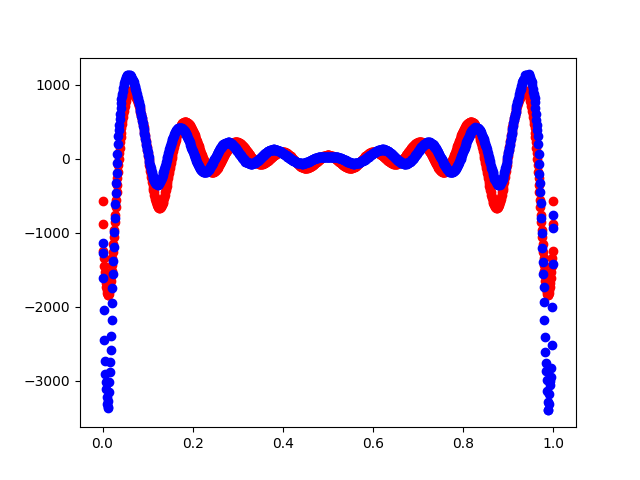
\includegraphics[width=6cm]{figure/model1_1000.png}
	\hspace{1cm}
	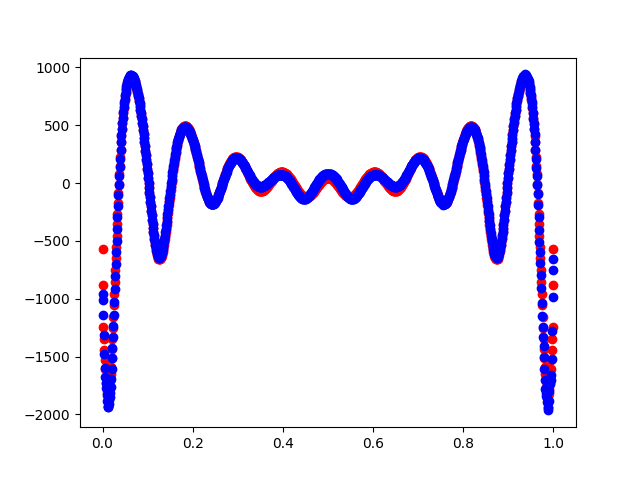
\includegraphics[width=6cm]{figure/model1_10000.png}
	\bicaption{中文题图}
	{English caption}
	\label{fig1}
\end{figure}

\begin{figure}[htp]
    \centering
    
\includegraphics[width=0.5\linewidth]{figure/attention.png}
    \bicaption{中文题图}{English caption}
    \label{fig:placeholder}
\end{figure}

\section{选题来源与背景}

特征值与特征向量问题是线性代数与矩阵理论中的核心内容之一，其数学表述为：对于给定的 $n$ 阶实对称矩阵 $A \in \mathbb{R}^{n \times n}$，寻找标量 $\lambda$ 和非零向量 $x \in \mathbb{R}^n$，使得
\[
Ax = \lambda x
\]
成立，其中 $\lambda$ 称为矩阵 $A$ 的特征值，$x$ 称为对应于 $\lambda$ 的特征向量。若进一步要求 $\|x\|_2 = 1$，则称 $x$ 为单位特征向量。

特征值问题的研究最早可追溯到 18 世纪欧拉（Euler）对刚体转动惯量主轴的研究，以及拉格朗日（Lagrange）和柯西（Cauchy）在力学系统稳定性分析中的工作。19 世纪，随着矩阵理论的建立（凯莱、西尔维斯特等人的贡献），特征值问题被纳入到统一的代数框架之中。20 世纪以来，随着量子力学、振动理论、控制论等学科的发展，特征值问题逐渐成为现代科学与工程计算中不可或缺的工具。

\section{选题目的与意义}

对于实对称矩阵，其特征值均为实数，且可按大小排序为
\[
\lambda_1 \leq \lambda_2 \leq \cdots \leq \lambda_n
\]
其中，最小特征值（第一特征值）$\lambda_1$ 与次最小特征值（第二特征值）$\lambda_2$ 具有特别重要的物理与应用意义：

在主成分分析（PCA）中，协方差矩阵的第一、第二主特征值对应数据方差最大的两个方向，是数据降维与可视化的基础；在谱图理论中，图拉普拉斯矩阵的第二小特征值（代数连通度，Fiedler 值）刻画了图的连通性，与图分割、社区发现密切相关；在结构动力学中，第一、第二阶固有频率（对应于特征值）决定了结构的主要振动模态；在网络分析（如 Google 的 PageRank 算法）中，主特征向量给出了网页的重要性排序。由瑞利商（Rayleigh quotient）理论可知，第一特征值满足极值刻画：
\[
\lambda_1 = \max_{x \neq 0} \frac{x^{\mathrm{T}} A x}{x^{\mathrm{T}} x}
\]
而第二特征值则由 Courant--Fischer 极小极大定理给出：
\[
\lambda_2 = \max_{\substack{x \neq 0 \\ x \perp v_1}} \frac{x^{\mathrm{T}} A x}{x^{\mathrm{T}} x}
\]
其中 $v_1$ 为第一特征值对应的特征向量。这一变分刻画为采用优化算法求解特征值提供了理论桥梁。

本研究将数值代数中的特征值问题与群体智能优化方法相结合，深化了对瑞利商变分原理的理解与应用，丰富了特征值求解的方法体系，为以优化视角处理代数问题提供了实例与思路。

应用意义：

基于 PSO 的方法不依赖矩阵的可微性与特殊结构，对于一些传统方法难以处理的非常规问题（如带复杂约束的广义特征值问题）具有潜在的适用性；算法的并行性良好，适合在现代多核与分布式计算环境下实现，便于扩展到大规模问题；第一、第二特征值在 PCA、谱聚类、图分割、振动分析等众多领域有直接应用，本研究的成果可为这些应用领域提供新的计算工具。

\section{国内外文献综述}

传统的特征值求解方法主要包括幂法（Power Method）、反幂法、QR 算法、Jacobi 方法、Lanczos 方法等。这些方法在精度和稳定性方面表现优异，但也存在一定局限：

幂法对特征值分布敏感，当 $|\lambda_1|$ 与 $|\lambda_2|$ 接近时收敛缓慢；QR 算法计算复杂度较高（$O(n^3)$），且对初值和矩阵结构有一定要求；部分方法在处理大规模稀疏矩阵或病态矩阵时面临数值不稳定问题。正是由于上述瑞利商所揭示的特征值问题与优化问题的等价性，使得将群体智能优化算法应用于特征值求解成为可能。粒子群优化算法（Particle Swarm Optimization, PSO）作为一种典型的群体智能方法，具有原理简单、参数少、全局搜索能力强、不依赖目标函数梯度信息等优点，为特征值问题提供了一条新的求解途径。

特征值问题的经典数值方法已发展得较为成熟。Golub 与 Van Loan 在其经典著作《Matrix Computations》中系统总结了 QR 算法、幂法、Lanczos 方法等的理论与实现。幂法及其变体（反幂法、移位幂法）由于实现简单，常用于求解主特征值；但当 $\lambda_1$ 与 $\lambda_2$ 的比值 $|\lambda_2 / \lambda_1|$ 接近 1 时，其收敛速度显著下降。

QR 算法是求解中小规模稠密矩阵全部特征值的标准方法，由 Francis 与 Kublanovskaya 于 20 世纪 60 年代提出，具有良好的数值稳定性。对于大规模稀疏对称矩阵，Lanczos 方法及其重正交化变体得到了广泛应用。此外，Davidson 方法、Jacobi-Davidson 方法在量子化学计算中求解极端特征值方面表现出色。

尽管这些方法体系完整、精度高，但它们大多基于矩阵分解或迭代收缩，在面对非标准的约束条件或非线性扩展时，往往需要重新设计算法。

粒子群优化算法由 Kennedy 与 Eberhart 于 1995 年首次提出，其灵感来源于鸟群觅食的群体行为。在标准 PSO 中，每个粒子 $i$ 的位置 $x_i$ 与速度 $v_i$ 按如下规则更新：
\begin{equation}
 v_i^{t+1} = w \cdot v_i^t + c_1 r_1 (p_i - x_i^t) + c_2 r_2 (g - x_i^t)   
\end{equation}
\[
x_i^{t+1} = x_i^t + v_i^{t+1}
\]
其中 $w$ 为惯性权重，$c_1, c_2$ 为学习因子，$r_1, r_2$ 为 $[0,1]$ 上的随机数，$p_i$ 为粒子的个体历史最优位置，$g$ 为群体全局最优位置。

为提升算法性能，学者们提出了诸多改进：Shi 与 Eberhart 引入惯性权重以平衡全局与局部搜索能力；Clerc 与 Kennedy 提出收缩因子（constriction factor）模型以保证算法收敛性；此后又出现了自适应 PSO、量子行为 PSO（QPSO）、混合 PSO 等多种变体。这些研究表明，PSO 在连续优化问题中具有良好的全局搜索能力，但也存在易陷入局部最优、后期收敛速度慢等问题。

将智能优化算法用于特征值求解的研究近年来逐渐增多。早期有学者利用神经网络（如 Hopfield 网络、递归神经网络）求解实对称矩阵的特征值与特征向量，将瑞利商作为能量函数构造动力系统。

在群体智能方面，已有研究将遗传算法（GA）、差分进化（DE）等用于求解最大/最小特征值。针对 PSO，部分文献探索了利用 PSO 求解主特征值的方法，其核心思想是将瑞利商作为适应度函数，在单位球面约束下搜索最优向量。这类研究验证了 PSO 求解特征值的可行性，但多数仅关注单个极端特征值，对于第二乃至更多特征值的连续求解、单位特征向量的约束处理以及正交约束的实现，仍有进一步研究的空间。

\section{研究内容}

本文的主要研究目的包括：

建立特征值问题的优化模型：基于瑞利商的极值特性以及 Courant--Fischer 定理，将第一、第二特征值及其单位特征向量的求解转化为带约束的优化问题；

设计基于 PSO 的求解算法：针对单位特征向量的约束条件 $\|x\|_2 = 1$ 与正交约束 $x \perp v_1$，设计相应的适应度函数与约束处理策略，构造可行的粒子群求解框架；

实现连续求解机制：在求得第一特征值与特征向量的基础上，通过收缩（deflation）或正交投影技术，连续求解第二特征值及其单位特征向量；

进行数值实验验证：通过与传统方法（如幂法、QR 算法）的对比，验证所提算法的有效性、精度与适用范围。

\begin{table}[!ht]
	\bicaption{中文图名}{english name}\label{tab:lable}
	\begin{tabular*}{\hsize}{@{}@{\extracolsep{\fill}}lllllllllllll@{}}
		\toprule
		$p_{t}$  &21  &22  &20  &15  &10  &8   &5   &10  &18  &10  &14  &18\\
		\midrule
		$c_{t}$  &5   &13  &10  &10  &10  &10  &10  &10  &10  &10  &10  &10\\
		$h_{t}$  &10  &5   &5   &5   &5   &5   &5   &5   &5   &5   &5   &5 \\
		$s_{t}$  &100 &100 &100 &100 &100 &100 &100 &100 &100 &100 &100 &100\\
		$d_{t}$  &30  &45  &50  &55  &45  &55  &90  &80  &90  &65  &80  &70 \\
		\bottomrule
	\end{tabular*}
\end{table}

\section{本章总结}

第一章，介绍选题背景、目的与意义、国内外文献综述以及本文的主要研究内容。
第二章，介绍平均相对误差的定义、数据拟合方法及数据预处理过程。
第三章，介绍分段拟合方法的实现过程、精度评估及剩余放电时间计算。
第四章，介绍通用模型的构建方法、精度评估及 55A 放电曲线的预测。
第五章，分析衰减特性并建立预测模型，预测不同衰减状态下剩余放电时间。

% ============================================================================
% 第 2 章 预备知识（转写自 chapter/chapsection/01Preliminaries.tex）
% ============================================================================
\chapter{预备知识}
我是预备知识

在离散数学中，图（Graph）是用于表示物体与物体之间存在某种关系的结构。数学抽象后的“物体”称作节点或顶点（英语：Vertex，node或point），节点间的相关关系则称作边。\upcite{bierlich2022comprehensive}在描绘一张图的时候，通常用一组点或小圆圈表示节点，其间的边则使用直线或曲线。

用$\mathbb{R}$和$\mathbb{R}^{n}$分别表示实数域和$n$维实数域. 对任意的实数$x \in \mathbb{R}$, $\lfloor x \rfloor$是向下取整函数，表示不大于$x$的最大整数，且$ \lfloor x \rfloor \leq x$；$\lceil x \rceil$是向上取整函数，表示不小于$x$的最小整数，且$\lceil x \rceil \geq x$.
 
\section{向量、矩阵和范数}
二维平面上的一点$P=(x,y)^{\top}$

\begin{lemma}\label{Lemma4EmYqK}
	假设$e_p,~p=1,2,\cdots,m$是$m$维单位矩阵的第$p$列和列向量$Y_{q} = \left( y_{1,q}, y_{2,q}, \cdots, y_{m,q} \right)^\top \in \mathbb{R}^{m}$, 且$y_{p,q} \neq 0$,  则
	\begin{equation*}
	 \left( e_1, \cdots,e_{p-1}, Y_{q}, e_{p+1}, \cdots, e_m \right)^{-1}  = 
	  	   		\begin{pmatrix} 
		  		1 	   & 0      & \cdots  & 0 			  & -\frac{y_{1,q}}{y_{p,q}}  	& 0 	& \cdots   & 0\\
		  		0 	   & 1      & \cdots  & 0 			  & -\frac{y_{2,q}}{y_{p,q}}  	& 0 	& \cdots   & 0\\
		  		\vdots & \vdots & \ddots  & \vdots 	      &  \vdots     	& \vdots  	& \ddots  & \vdots\\
		  		0      & 0      & \cdots  & 1  			  & -\frac{y_{p-1,q}}{y_{p,q}}  	& 0 	& \cdots   & 0\\	  		
		  		0      & 0      & \cdots  & 0  			  & \frac{1}{y_{p,q}}  	& 0 	& \cdots   & 0\\
		  		0      & 0      & \cdots  & 0  			  & -\frac{y_{p+1,q}}{y_{p,q}}  	& 1 	& \cdots   & 0\\
		  		\vdots & \vdots & \ddots  & \vdots  	  & \vdots  		& \vdots  	& \ddots   & \vdots\\	
		  		0      & 0      & \cdots  & 0  			   & -\frac{y_{m,q}}{y_{p,q}}     & 0     & \cdots   & 1\\	  		
			\end{pmatrix} .
	\end{equation*}
\end{lemma}

\section{开集和闭集}
以$x \in \mathbb{R}^{n}$为球心，$r > 0$为半径的开球记为 
\begin{equation*}
    \mathcal{B}\left(x,r\right) \triangleq \left\{ y \in \mathbb{R}^{n} : \Vert y - x \Vert_{2} < r \right\}
\end{equation*}
和相应的闭球
\begin{equation*}
    \overline{\mathcal{B}}\left(x,r\right) \triangleq \left\{ y \in \mathbb{R}^{n} : \Vert y - x \Vert_{2} \leq r \right\}.
\end{equation*}

\begin{definition}\label{Chapter0Open}
    设非空集合$\mathcal{S} \subseteq \mathbb{R}^{n}$. 若对任意的$x \in \mathcal{S}$, 总存在$r > 0$, 使得$\mathcal{B}\left(x,r\right) \subseteq \mathcal{S}$, 则称$\mathcal{S}$为\textbf{开集}. \textbf{补集}$~\mathcal{S}^{\mathrm{c}} \triangleq \left\{ x \in \mathbb{R}^{n} : x \notin \mathcal{S} \right\}$为开集的集合$\mathcal{S}$称为\textbf{闭集}，其中\textbf{补集}$~\mathcal{S}^{\mathrm{c}}$也被记为$~\overline{\mathcal{S}}$.
\end{definition}

显然地，开球$\mathcal{B}\left(x,r\right)$和闭球$\overline{\mathcal{B}}\left(x,r\right)$分别是开集和闭集. 包含点$x \in \mathbb{R}^{n}$的开集称为$x$的一个\textbf{邻域}. 全空间$\mathbb{R}^{n}$和空集$\emptyset$既是开集又是闭集. 进一步地，
\begin{itemize}
 \setlength{\itemsep}{0pt}
 \setlength{\parsep}{0pt}
 \setlength{\parskip}{0pt}
     \item[$(1)$] 有限个开集$S_i(i=1,\cdots,m)$的交集$\bigcap_{i=1}^{m}S_i$是开集，任意个开集$S_i(i \in \mathcal{I} )$的并集$\bigcup_{i \in \mathcal{I}}S_i$是开集，其中$\mathcal{I}$为有限或无限的指标集合；
     \item[$(2)$] 有限个闭集$S_i(i=1,\cdots,m)$的并集$\bigcup_{i=1}^{m}S_i$是闭集，任意个闭集$S_i(i \in \mathcal{I} )$的交集$\bigcap_{i \in \mathcal{I}}S_i$是闭集，其中$\mathcal{I}$为有限或无限的指标集合.
\end{itemize}

给定一个非空集合$\mathcal{S} \subseteq \mathbb{R}^{n}$与点$x \in \mathcal{S}$, 若存在$r > 0$, 使得$\mathcal{B}\left(x,r\right) \subseteq \mathcal{S}$, 则称$x$为$\mathcal{S}$的\textbf{内点}. 非空集合$\mathcal{S}$中所有\textbf{内点}构成的集合称为$\mathcal{S}$的\textbf{内部},记为$\mathrm{int}\,\mathcal{S}$. 显然，$\mathrm{int}\,\mathcal{S}$是开集，这是因为在$\mathrm{int}\,\mathcal{S}$中的任何一个点，都可找到一个属于$\mathrm{int}\,\mathcal{S}$的开球. 另外，称包含$\mathcal{S}$的最小闭集，即所有包含$\mathcal{S}$的闭集的交集，为$\mathcal{S}$的\textbf{闭包}, 记为$\mathrm{cl}\,\mathcal{S}$. 属于$\mathrm{cl}\,\mathcal{S}$但不属于$\mathrm{int}\,\mathcal{S}$的所有点构成的集合称为$\mathrm{int}\,\mathcal{S}$的边界，记为$\mathrm{bd}\,\mathcal{S}$. 如果存在一个充分大的数$r > 0$, 使得$\mathcal{S} \subseteq \mathcal{B}\left(0,r\right)$, 则称$\mathcal{S}$是\textbf{有界}. 进一步地，称\textbf{有界闭集}$\mathcal{S}$为\textbf{紧集}. 注意，此处的\textbf{紧集}的定义只适合有限维空间.

\section{凸集和凸函数}
图中的边可以是有方向或没有方向的。例如在一张图中，如果节点表示聚会上的人，而边表示两人曾经握手，则该图就是没有方向的，因为甲和乙握过手也意味着乙一定和甲握过手。相反，如果一条从甲到乙的边表示甲欠乙的钱，则该图就是有方向的，因为“曾经欠钱”这个关系不一定是双向的。前一种图称为无向图，后一种称为有向图。

\begin{definition}\label{Chapter0Cone}
    设非空集合$\mathcal{C} \subseteq \mathbb{R}^{n}$. 如果满足对任意的$x \in \mathcal{C}$和$\alpha \in [0,+\infty)$, 都有$\alpha x \in \mathcal{C}$, 则称$\mathcal{C}$为\textbf{锥}.
\end{definition}

从锥的定义 \ref{Chapter0Cone} 可知，锥$\mathcal{C}$是包含所有以原点为起点，并通过$\mathcal{C}$中一点的射线的集合. 当锥$\mathcal{C}$是凸集，称之为\textbf{凸锥}；当锥$\mathcal{C}$是闭集时，称之为\textbf{闭锥}；当锥$\mathcal{C}$既是凸集又是闭集时，则称之为\textbf{闭凸锥}.

\section{梯度、Hessian矩阵和Jacobi矩阵}

\begin{definition}[梯度]
    给定函数 $f: \mathbb{R}^n \to \mathbb{R}$，且$f$在点$x$的一个邻域内有定义，若存在向量 $g \in \mathbb{R}^n$ 满足
	\begin{equation*}
	   \lim_{p \to 0} \frac{f(x+p) - f(x) - g^{\mathrm{T}} p}{\|p\|} = 0, 
	\end{equation*}
    其中 $\| \cdot \|$ 是任意的向量范数，就称 $f$ 在点 $x$ 处\textup{Fr\'{e}chet} 可微．此时 $g$ 称为 $f$ 在点 $x$ 处的\textbf{梯度}，记作 $\nabla f(x)$．
	如果对区域 $D$ 上的每一个点 $x$ 都有 $\nabla f(x)$ 存在，则称 $f$ 在 $D$ 上\textup{Fr\'{e}chet}可微．
\end{definition}

若 $f$ 在点 $x$ 处的梯度存在，在定义式中令 $p = \varepsilon e_i$，$e_i$是第$i$个分量为$1$的单位向量，可知 $\nabla f(x)$ 的第 $i$ 个分量为 $\dfrac{\partial f(x)}{\partial x_i}$．因此 
\begin{equation*}
   \nabla f(x) = \left[ \frac{\partial f(x)}{\partial x_1}, \frac{\partial f(x)}{\partial x_2}, \cdots, \frac{\partial f(x)}{\partial x_n} \right]^{\mathrm{T}}.
\end{equation*}
 
\begin{definition}[Hessian矩阵]
	如果函数$f(x): \mathbb{R}^n \to \mathbb{R}$在点$x$处的二阶偏导数
		$\frac{\partial^2 f(x)}{\partial x_i \partial x_j}$ $i,j
		=1,2,\cdots,n$都存在，则$f$ 在点 $x$ 处的\textup{Hessian}矩阵为:
		\[ 
		\mathbf{H} = \mathbf{H}_f \left( x\right)  \triangleq \nabla^2 f(x) =
		\begin{bmatrix}
			\dfrac{\partial^2 f(x)}{\partial x_1^2}            & \dfrac{\partial^2 f(x)}{\partial x_1 \partial x_2} & \dfrac{\partial^2 f(x)}{\partial x_1 \partial x_3} & \cdots & \dfrac{\partial^2 f(x)}{\partial x_1 \partial x_n} \\
			\dfrac{\partial^2 f(x)}{\partial x_2 \partial x_1} & \dfrac{\partial^2 f(x)}{\partial x_2^2}            & \dfrac{\partial^2 f(x)}{\partial x_2 \partial x_3} & \cdots & \dfrac{\partial^2 f(x)}{\partial x_2 \partial x_n} \\
			\vdots                                             & \vdots                                             & \vdots                                             &        & \vdots                                             \\
			\dfrac{\partial^2 f(x)}{\partial x_n \partial x_1} & \dfrac{\partial^2 f(x)}{\partial x_n \partial x_2} & \dfrac{\partial^2 f(x)}{\partial x_n \partial x_3} & \cdots & \dfrac{\partial^2 f(x)}{\partial x_n^2}            
		\end{bmatrix}
		 \in \mathbb{R}^{n \times n}.
		\]
		特别地，Hessian矩阵的第$i$行第$j$列的元素为： $ \mathbf{H}_{ij} = \left(\mathbf{H}_f\left( x\right)  \right)_{ij} = \dfrac{\partial^2 f(x)}{\partial x_i \partial x_j}.$
\end{definition}

% ============================================================================
% 第 3 章 数据预处理（转写自 chapter/chapsection/02Dataproc.tex）
% ============================================================================
\chapter{数据预处理}

我是主要结果，章名换成您要研究的内容，此章要分几个小节，每个小节是要处理的问题.

\section{数据的来源与描述}

\section{数据的预处理}

\subsection{缺失值和异常值处理}

\subsection{归一化和标准化}

\subsection{非数值数据的编码}

\section{处理后的数据分析}

\subsection{数据分布情形}

% ============================================================================
% 第 4 章 主要内容（转写自 chapter/chapsection/03myresults.tex）
% ============================================================================
\chapter{主要内容}

我是主要结果，章名换成您要研究的内容，此章要分几个小节，每个小节是要处理的问题.

\section{向量值函数的微分}

\begin{algorithm}[th!]
\SetAlgoLined
\KwIn{Matrix $\mathbf{A} \in \mathbb{R}^{n \times n}$, number of particles $N$, max iterations $T$, inertia weight $w$, learning factors $c_1, c_2$.}

\textbf{Initialize}: For each particle $i = 1, \dots, N$:
\begin{itemize}
    \item Position $\mathbf{x}_i^0 \sim \mathcal{N}(0, 1)$ (normalized: $\mathbf{x}_i^0 \gets \mathbf{x}_i^0 / \|\mathbf{x}_i^0\|_2$).
    \item Velocity $\mathbf{v}_i^0 = \mathbf{0}$.
    \item Personal best $\mathbf{p}_i^0 = \mathbf{x}_i^0$, best value $f_i^0 = \text{Rayleigh}(\mathbf{x}_i^0)$.
\end{itemize}
Global best $\mathbf{g}^0 = \text{argmin}_{\mathbf{p}_i^0} \{f_1^0, \dots, f_N^0\}$.

\While{ $k < T$}{
 \begin{itemize}
 \item[(1)] \textbf{Update Velocity}: For each particle $i$:
    \[
    \mathbf{v}_i^{k+1} = w \mathbf{v}_i^k + c_1 r_1 (\mathbf{p}_i^k - \mathbf{x}_i^k) + c_2 r_2 (\mathbf{g}^k - \mathbf{x}_i^k)
    \]
    where $r_1, r_2 \sim U(0, 1)$.

 \item[(2)] \textbf{Update Position}: For each particle $i$:
    \[
    \mathbf{x}_i^{k+1} = \mathbf{x}_i^k + \mathbf{v}_i^{k+1}
    \]
    (Optional: Normalize $\mathbf{x}_i^{k+1} \gets \mathbf{x}_i^{k+1} / \|\mathbf{x}_i^{k+1}\|_2$)

 \item[(3)] \textbf{Update Best Positions}: Calculate fitness $f_i^{k+1} = \frac{(\mathbf{x}_i^{k+1})^\top \mathbf{A} \mathbf{x}_i^{k+1}}{(\mathbf{x}_i^{k+1})^\top \mathbf{x}_i^{k+1}}$:
    \begin{itemize}
        \item If $f_i^{k+1} < f_i^k$, then $\mathbf{p}_i^{k+1} = \mathbf{x}_i^{k+1}$ and $f_i^k = f_i^{k+1}$.
        \item If $f_i^{k+1} < \text{Rayleigh}(\mathbf{g}^k)$, then $\mathbf{g}^{k+1} = \mathbf{x}_i^{k+1}$.
    \end{itemize}

 \item[(4)] Update $k = k + 1.$
 \end{itemize}
}
\KwOut{ Minimal eigenvalue $\lambda \approx \text{Rayleigh}(\mathbf{g}^T)$ and eigenvector $\mathbf{x} = \mathbf{g}^T$.}
\AlgoBiCaption{粒子群优化算法求解最小特征值}{Particle Swarm Optimization for eigenvalue problem}\label{A:pso}
\end{algorithm}

\section{Jacobian矩阵}

\begin{algorithm}[th!]
\SetAlgoLined
    \KwIn{ 
        矩阵 $\mathbf{A} \in \mathbb{R}^{n \times n}$, 
        粒子数量 $N$, 
        最大迭代次数 ${\tt IterMax}$, 
        惯性权重 $w$, 
        加速因子 $c_1$ 和 $c_2$, 
        容差 $\varepsilon = 10^{-6}$
    }

    \While{ $k < {\tt IterMax}$ or $\frac{\Vert \mathbf{g}^{k} - \mathbf{g}^{k-1} \Vert_2}{ \Vert \mathbf{g}^{k} \Vert_2} >\varepsilon$ }{
        \begin{itemize}
        \item[(1)] \textbf{计算适应度并更新个体最优} \\
            对于每个粒子 $i = 1, 2, \dots, N$：
            \[
                f_i^k = (\mathbf{x}_i^k)^\top \mathbf{A} \mathbf{x}_i^k
            \]
            若 $f_i^k < pbest_i$，则更新：
            \[
                pbest_i \leftarrow f_i^k, \quad \mathbf{p}_i \leftarrow \mathbf{x}_i^k
            \]

        \item[(2)] \textbf{更新全局最优} \\
            找到当前最优粒子：
            \[
                i^* = \arg\min_{1 \leq i \leq N} pbest_i
            \]
            更新全局最优位置和值：
            \[
                \mathbf{g}^k \leftarrow \mathbf{p}_{i^*}, \quad gbest \leftarrow pbest_{i^*}
            \]

        \item[(3)] \textbf{更新速度与位置} \\
            对每个粒子 $i = 1, 2, \dots, N$ 执行：
            \[
            \begin{cases}
                \mathbf{v}_i^{k+1} &= w \mathbf{v}_i^k + c_1 r_1 (\mathbf{p}_i - \mathbf{x}_i^k) + c_2 r_2 (\mathbf{g}^k - \mathbf{x}_i^k) \\
                \mathbf{x}_i^{k+1} &= \mathbf{x}_i^k + \mathbf{v}_i^{k+1}
            \end{cases}
            \]
            \textbf{单位化约束}：
            \[
                \mathbf{x}_i^{k+1} \leftarrow \frac{\mathbf{x}_i^{k+1}}{\Vert \mathbf{x}_i^{k+1} \Vert_2}
            \]

        \item[(4)] 更新 $k = k + 1$
        \end{itemize}
    }
    \KwOut{ 
        返回最小特征值 $gbest$ 及其对应的单位特征向量 $\mathbf{g}^k$.
    }
    \AlgoBiCaption{粒子群优化算法求解最小特征值}{Particle Swarm Optimization for Minimum Eigenvalue}\label{alg:pso_mineig}
\end{algorithm}

\section{向量值函数的性质}
\begin{itemize}
 \setlength{\itemsep}{0pt}
 \setlength{\parsep}{0pt}
 \setlength{\parskip}{0pt}
	\item[$(1)$] 设函数$f(x): \mathbb{R}^n \to \mathbb{R}$在点$x$处的Hessian矩阵存在，则
	\begin{equation*}
		\mathbf{H}_f\left( x\right)  = \left( \mathbf{J}_{\nabla f}\left( x\right)  \right)^\top.
	\end{equation*}
	\item[$(2)$] 设函数$f(x): \mathbb{R}^n \to \mathbb{R}$在点$x$处的一阶梯度存在，对于$\theta \in [ 0,1]$和$x,y \in \mathrm{dom}(f)$, 则
	\begin{equation*}
		\dfrac{\partial f\left( x + \theta (y-x) \right) }{\partial \theta } = \nabla f^\top \left( x + \theta (y-x) \right) \left( y - x \right) .
	\end{equation*}
	\item[$(3)$] 设$\mathbf{F} : \mathbb{R}^{n} \rightarrow \mathbb{R}^{m}$和$\mathbf{H} : \mathbb{R}^{n} \rightarrow \mathbb{R}^{n}$的Jacobian矩阵都存在，则其复合函数
 $\Phi (x) = \left( \mathbf{F} \circ \mathbf{H} \right) (x) = \mathbf{F} \left( \mathbf{H} (x) \right)$的Jacobian矩阵为
	\begin{equation*}
		\mathbf{J}_{\Phi}\left( x \right) = \dfrac{\partial \mathbf{F} \left( \mathbf{H} \left( x \right) \right) }{\partial x} = \mathbf{J}_{\mathbf{F}}\left( \mathbf{H} \left( x \right) \right) \cdot \mathbf{J}_{\mathbf{H}}\left( x \right).
	\end{equation*}
 	\item[$(4)$] 设$\mathbf{F} : \mathbb{R}^{n} \rightarrow \mathbb{R}^{m}$和$f : \mathbb{R}^{n} \rightarrow \mathbb{R}$的Jacobian矩阵和梯度都存在，令$\Psi (x) = f(x) \mathbf{F}(x) $,则
	\begin{equation*}
		\mathbf{J}_{\Psi}\left( x \right) = \dfrac{\partial  \left( f(x) \mathbf{F}(x) \right) }{\partial x} = f(x) \mathbf{J}_{F}(x) + \mathbf{F}(x) \nabla^{\top} f(x)  .
	\end{equation*}
  	\item[$(5)$] 设$\mathbf{F} : \mathbb{R}^{n} \rightarrow \mathbb{R}^{m}$和$\mathbf{G}: \mathbb{R}^{n} \rightarrow \mathbb{R}^{m}$的Jacobian矩阵都存在，则其内积
   \begin{equation*}
       \langle \mathbf{F}(x), \mathbf{G}(x) \rangle \triangleq \sum_{i=1}^{m} f_{i}(x) g_{i}(x),~\forall x \in \mathbb{R}^{n}
   \end{equation*}
   其中$f_i,g_i : \mathbb{R}^{n} \rightarrow \mathbb{R}$,的导数为
	\begin{equation*}
		\nabla \left( \langle \mathbf{F}(x), \mathbf{G}(x) \rangle \right) = \mathbf{F}^{\top}(x) \mathbf{J}_{\mathbf{G}}(x) + \mathbf{G}^{\top}(x) \mathbf{J}_{\mathbf{F}}(x).
	\end{equation*}
  	\item[$(6)$] 设$\mathbf{F} : \mathbb{R} \rightarrow \mathbb{R}^{3}$和$\mathbf{G}: \mathbb{R} \rightarrow \mathbb{R}^{3}$的Jacobian矩阵都存在，则其叉积$\mathbf{F} \times \mathbf{G} : \mathbb{R} \rightarrow \mathbb{R}^{3}$的Jacobian矩阵为
	\begin{equation*}
		\mathbf{J}_{ \mathbf{F} \times \mathbf{G} } (t)  = \mathbf{J}_{\mathbf{F}}(t) \times \mathbf{G}(t) + \mathbf{F}(t) \times \mathbf{J}_{\mathbf{G}}(t).
	\end{equation*}
\end{itemize}
          % 载入正文各章汇总文件（内含绪论及各主体章节）

  % --------------------------------------------------------------------------
  % 3.4 后置部分：结论、参考文献、致谢与附录
  % 规范要求：结论、参考文献、致谢、附录均单独起页、不加章号、编入目录，
  %           继续沿用正文页眉与连续的阿拉伯数字页码（不重新从 1 开始）
  % --------------------------------------------------------------------------
  \backmatter                                   % 切换至后置模式：关闭后续 \chapter 的章节编号，但保持阿拉伯页码连续递增
  % -*- coding=utf-8 -*-
\chapter{结论}
我是结论我是结论我是结论我是结论我是结论我是结论我是结论我是结论我是结论我是结论我是结论我是结论我是结论我是结论我是结论我是结论我是结论我是结论我是结论我是结论我是结论我是结论        % 载入结论（作为正文最后一章单独排写，不加章号，自动计入目录）
  % -*- coding=utf-8 -*-
\nocite{*}
\printbibliography[title=参考文献,heading=bibintoc]
%\addcontentsline{toc}{chapter}{参考文献}
%%%%%%%%%%%%%%%%%%%%%%%%%%%%%%%%%%%%%%%%%%%%%%%%%%%%%%
% BibTeX  
% \bibliographystyle{unsrt}
% plain-此格式的参考文献的条目的编号是按照作者的字母顺序
% unsrt – 基本上跟 plain 类型一样，此格式的参考文献的条目的编号是按照引用的顺序，而不是按照作者的字母顺序
% alpha – 类似于 plain 类型，当参考文献的条目的编号基于作者名字和出版年份的顺序
% abbrv – 缩写格式
%\bibliographystyle{plain}
%\bibliography{refs.bib}

         % 载入参考文献（基于 biblatex + gb7714-2025，五号宋体，自动计入目录）
  % -*- coding=utf-8 -*-
\chapter{致谢}
我是致谢            % 载入致谢（置于参考文献之后、附录之前，不加章号，自动计入目录）
  % -*- coding=utf-8 -*-
\chapter{附录}

\section*{一、处理碰撞事例的Python代码}
%\begin{lstlisting}[language={python}, basicstyle = \ttfamily,breaklines = true, caption={Python 源代码}, label=code_1]
\begin{lstlisting}[language=python,caption={模拟退火算法},label=Code:101]
kk=2;
[mdd,ndd]=size(dd);
while ~isempty(V)
    [tmpd,j]=min(W(i,V));tmpj=V(j);
for k=2:ndd
    [tmp1,jj]=min(dd(1,k)+W(dd(2,k),V));
    tmp2=V(jj);tt(k-1,:)=[tmp1,tmp2,jj];
end
    tmp=[tmpd,tmpj,j;tt];[tmp3,tmp4]=min(tmp(:,1));
if tmp3==tmpd, ss(1:2,kk)=[i;tmp(tmp4,2)];
 \end{lstlisting}
 
 \newpage
 
 \section*{二、处理碰撞事例的Julia代码}
\begin{lstlisting}[language=matlab,caption={模拟退火算法},label=Code:102]
using LinearAlgebra
using Random

"""
PSO求解最小特征值及特征向量
A: 对称矩阵
n_particles: 粒子数量
max_iter: 最大迭代次数
"""
function pso_min_eigen(A::Matrix{Float64}; n_particles=50, max_iter=200)
    n = size(A, 1)

    # 定义目标函数：瑞利商 f(x) = (x'Ax) / (x'x)
    function rayleigh_quotient(x)
        return (x' * A * x) / (x' * x)
    end

    # 初始化粒子位置 (随机单位向量方向) 和速度
    particles = [randn(n) for _ in 1:n_particles]
    velocities = [zeros(n) for _ in 1:n_particles]

    # 个体最优位置及其适应度
    pbest_pos = copy(particles)
    pbest_val = [rayleigh_quotient(p) for p in particles]

    # 全局最优
    gbest_idx = argmin(pbest_val)
    gbest_pos = copy(pbest_pos[gbest_idx])
    gbest_val = pbest_val[gbest_idx]

    # 超参数
    w = 0.5   # 惯性权重
    c1 = 1.5  # 个体学习因子
    c2 = 1.5  # 全局学习因子

    for _ in 1:max_iter
        for i in 1:n_particles
            # 更新速度
            velocities[i] = w * velocities[i] + 
                            c1 * rand() * (pbest_pos[i] - particles[i]) + 
                            c2 * rand() * (gbest_pos - particles[i])

            # 更新位置
            particles[i] += velocities[i]

            # 计算适应度
            val = rayleigh_quotient(particles[i])

            # 更新个体最优
            if val < pbest_val[i]
                pbest_val[i] = val
                pbest_pos[i] = copy(particles[i])

                # 更新全局最优
                if val < gbest_val
                    gbest_val = val
                    gbest_pos = copy(particles[i])
                end
            end
        end
    end

    # 返回结果：特征值与单位特征向量
    return gbest_val, gbest_pos / norm(gbest_pos)
end

# --- 测试 ---
Random.seed!(123)
A = rand(5, 5)
A = A' * A # 构造对称正定矩阵
λ, v = pso_min_eigen(A)

println("PSO计算的最小特征值: ", λ)
println("对比线性代数库计算: ", minimum(eigvals(A)))
println("单位特征向量: ", v)
\end{lstlisting}

           % 载入附录（非必要补充部分，置于全文末尾，不加章号，自动计入目录）

\end{document}
